\subsection{Concept Summary}

Table \ref{table:concept_summary} summarizes the two primary subsystems identified for the WaterFront Robot; the robot leg topology and chassis, and solar panel mounting.
The selected solution from each subsystem is framed by a rectangular form.
Concept 2, the crab, was selected for the robot chassis and leg topology, and the Concept 3, the direct solar cell mounting, was selected for the solar panel mounting.

\begin{center}
    \setlength{\fboxrule}{4pt}
    \setlength{\fboxsep}{0pt}
    \begin{longtable}{| m{2cm} | p{4cm} | p{4cm} |  p{4cm} |}
        \caption{Summary of concepts, broken down by sub-function}
        \label{table:concept_summary}
         \\ \hline
         & \multicolumn{3}{c|}{Concepts}
         \\ \hline
          & 1 & 2 & 3
         \\ \hline
         Robot and Legs & 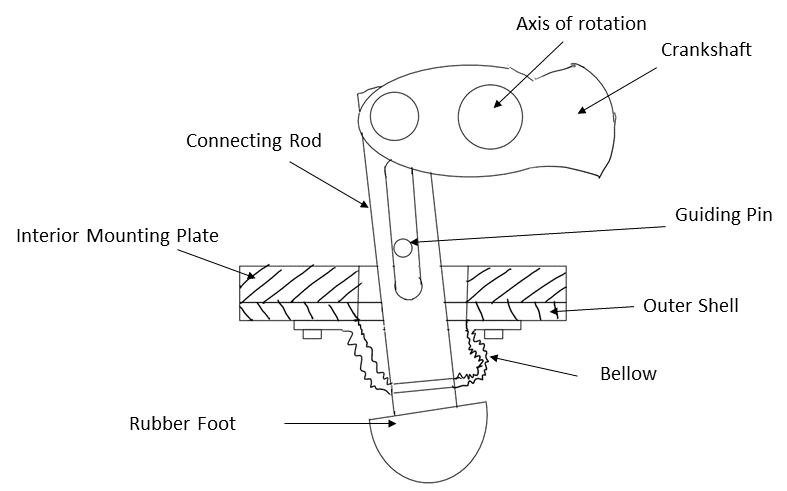
\includegraphics[width=4cm]{3_DesignConcepts/img/C1/Concept.PNG} & \fbox{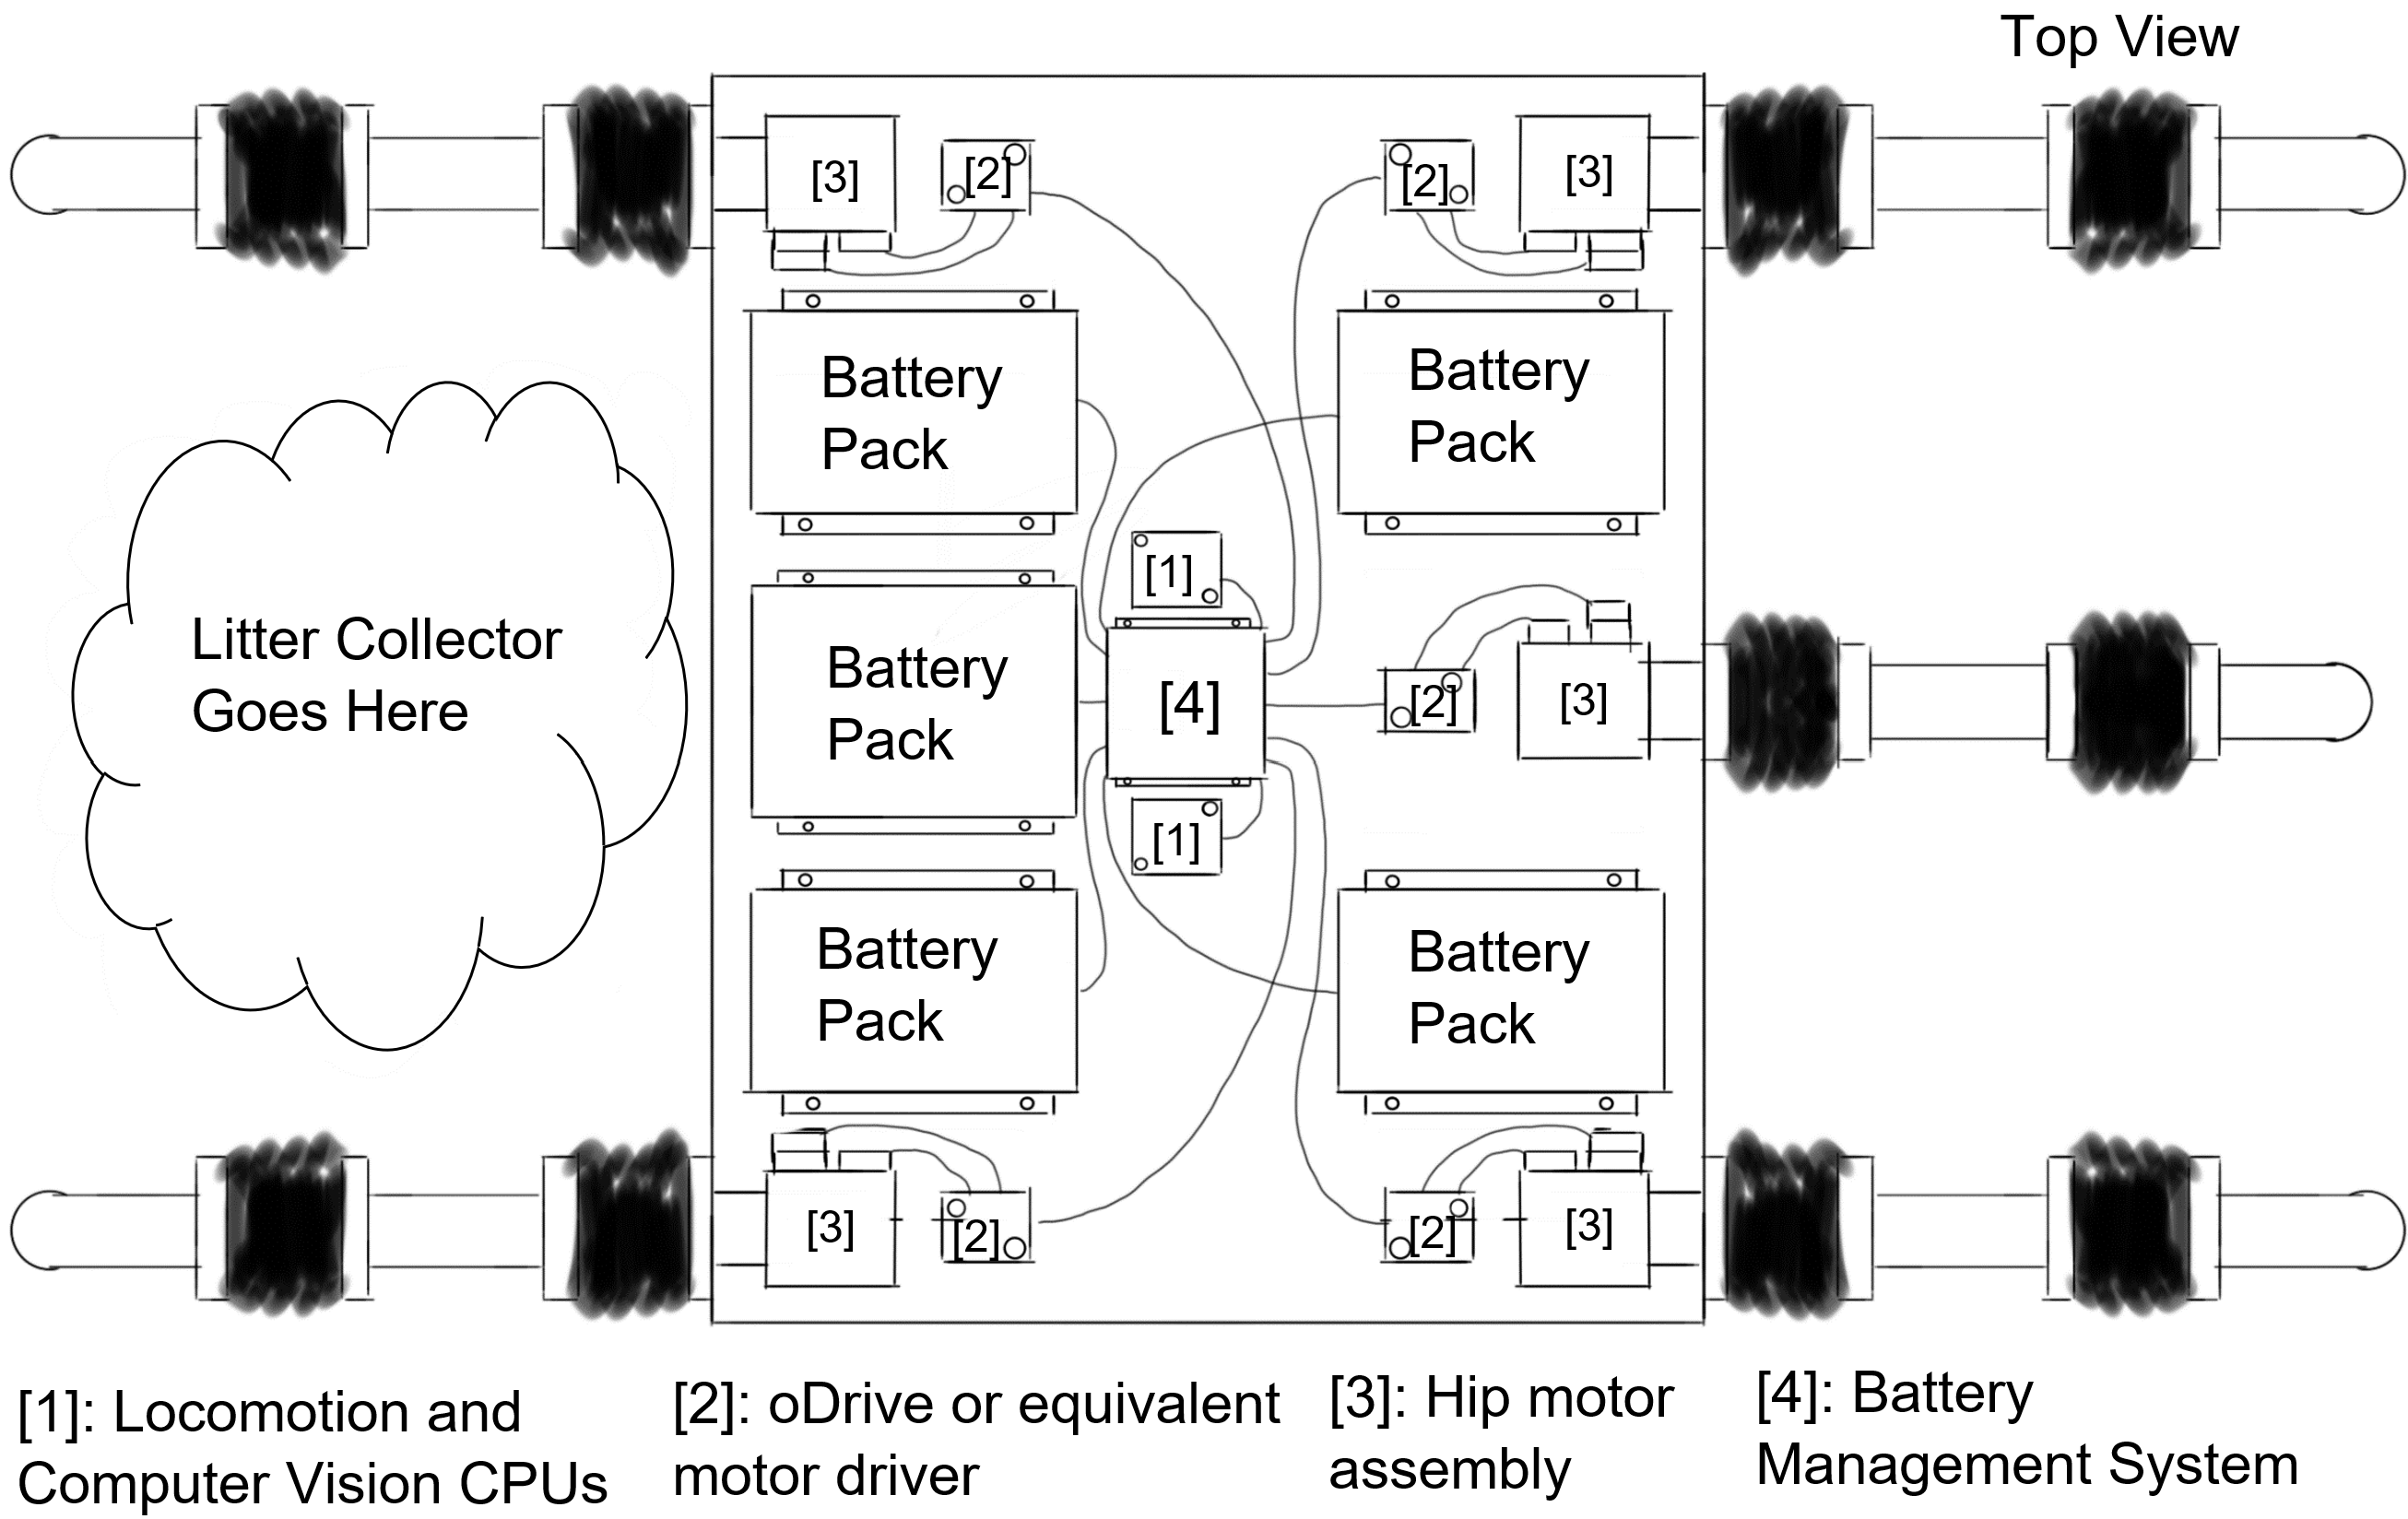
\includegraphics[width=4cm]{3_DesignConcepts/img/Crab/crab_top_view.png}} & 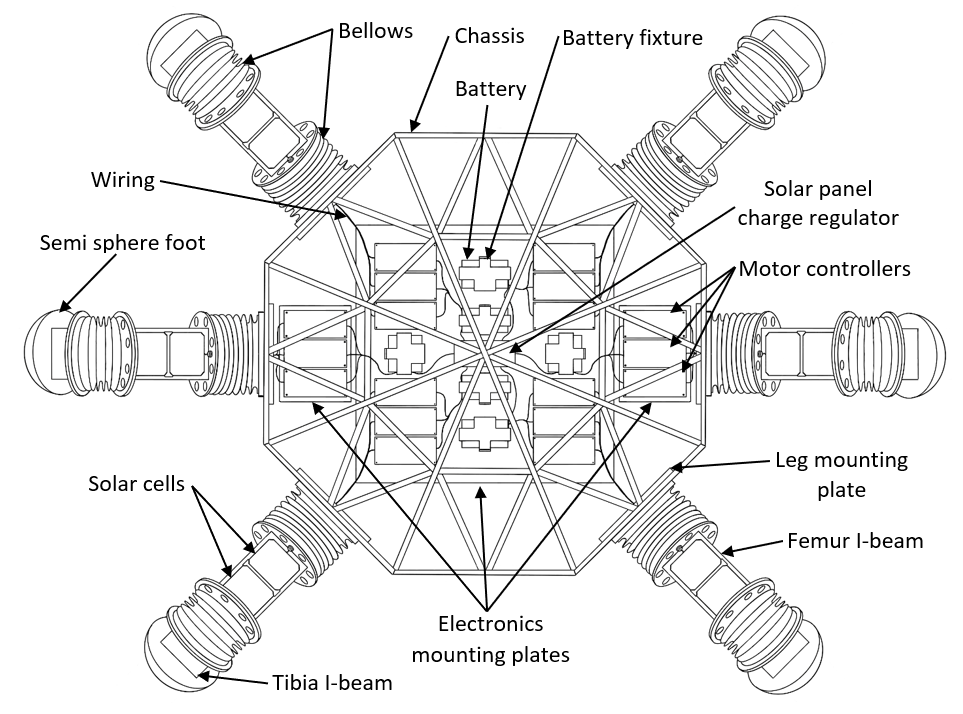
\includegraphics[width=4cm]{3_DesignConcepts/img/C3/overview_ann.PNG}
         \\ \hline
         Solar Panels & 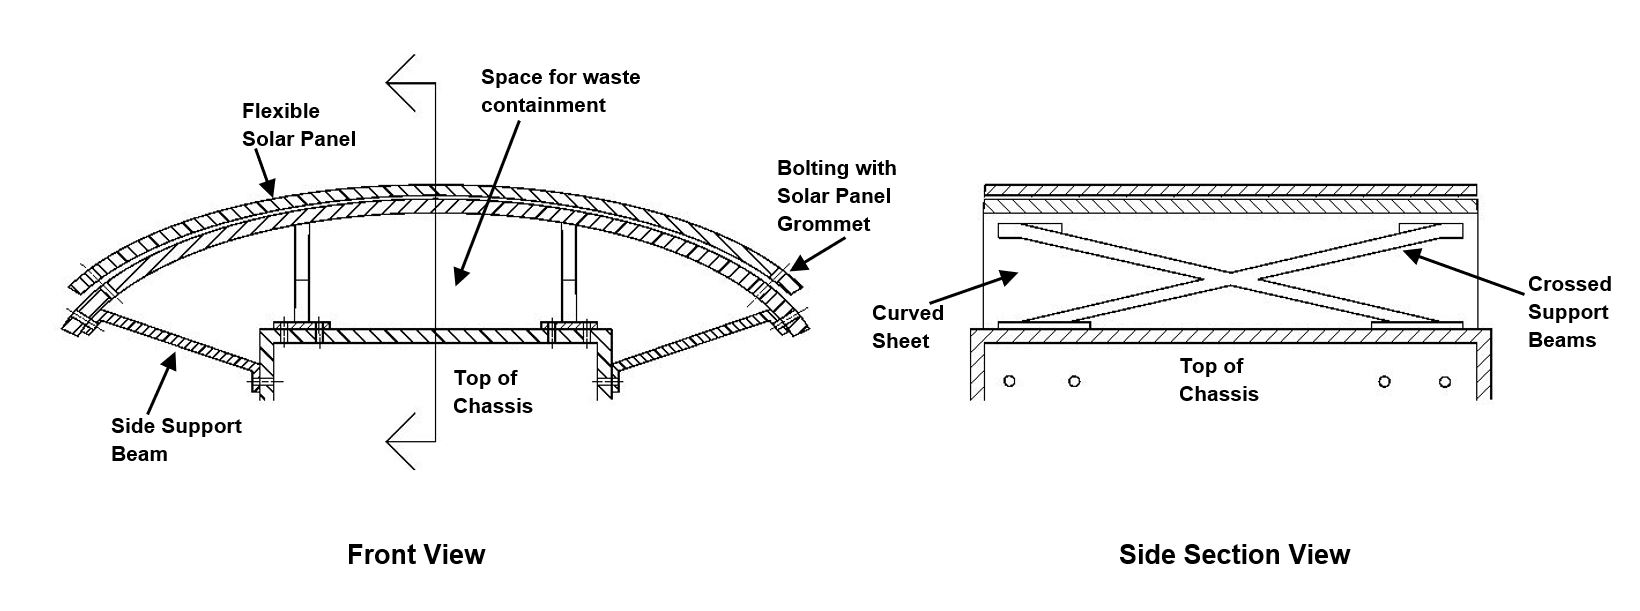
\includegraphics[width=4cm]{3_DesignConcepts/img/Solar/solar_roof.JPG} & 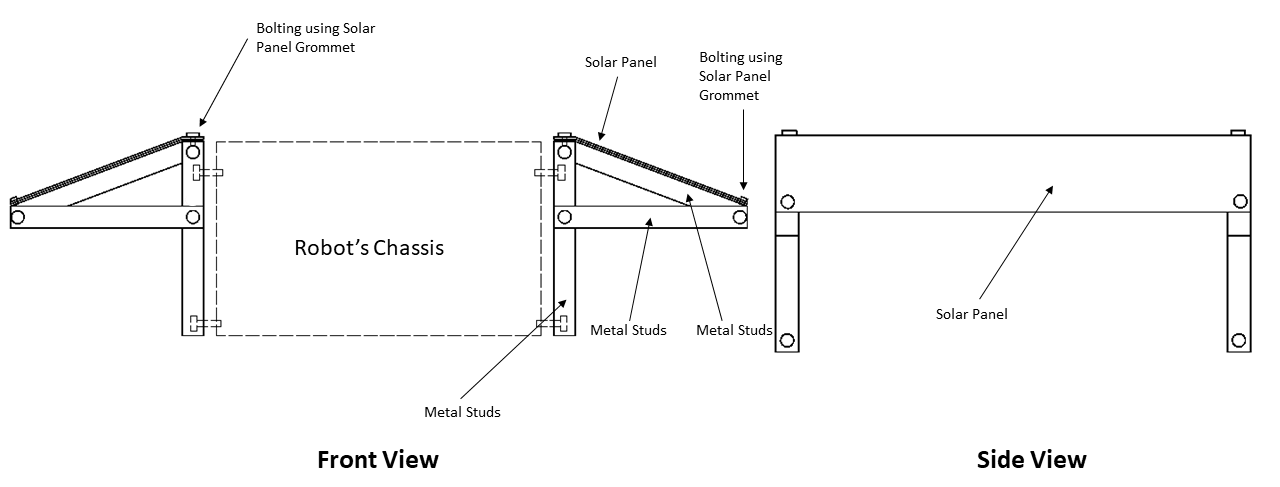
\includegraphics[width=4cm]{3_DesignConcepts/img/Solar/SolarSidePanel.png} & \fbox{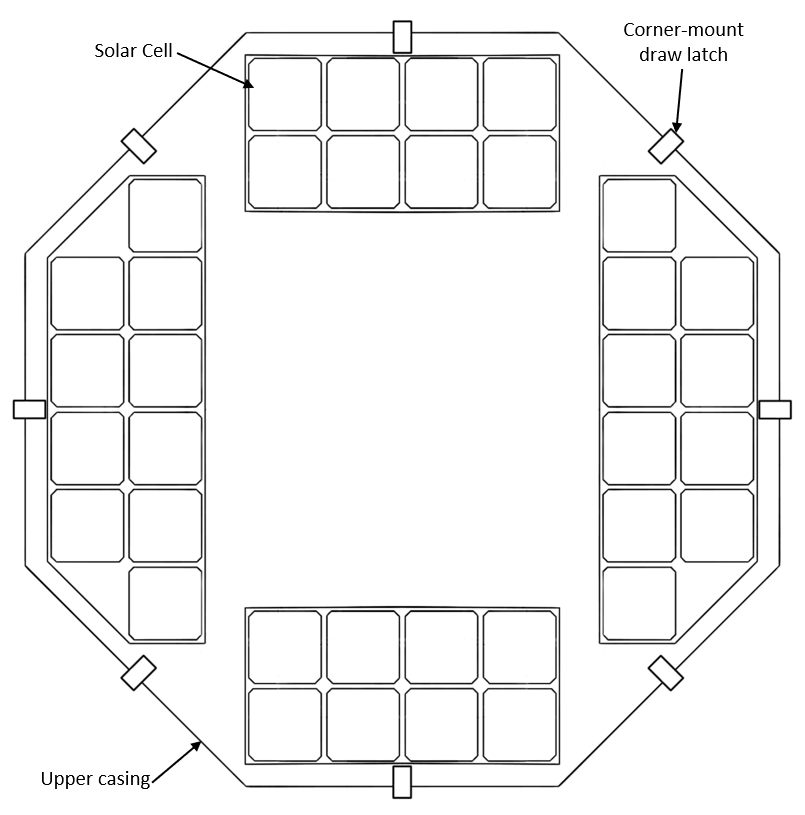
\includegraphics[width=3cm]{3_DesignConcepts/img/C3/solarcells_ann.PNG}}
         \\ \hline
    \end{longtable}
\end{center}